As discussed in the previous chapter, most of the solutions found in the literature rely on deep learning models. However, these models have a significant drawback: they are very complex and with a lot of parameters, meaning they excel at predicting the model's output, but are not equally suitable for explaining the phenomenon. Indeed, deep learning model can be seen as black-box model. We can use packages such as Shap, shown in Fig. \ref{fig:shap}, available as a Python package. SHAP (SHapley Additive exPlanations) utilizes game theory principles to explain the outputs of any machine learning model. It bridges the gap between optimal contribution distribution and localized explanations by employing the traditional Shapley values from game theory, along with their associated extensions as described by \citeauthor{lundberg_unified_2017} (2017).
\begin{figure}
    \centering
    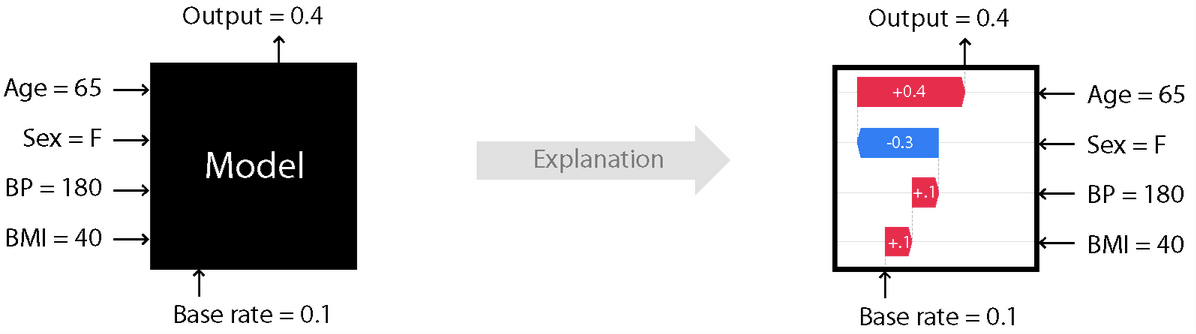
\includegraphics[width=0.7\textwidth]{Images/shap.png}
    \caption[SHAP python package.]{Example of the SHAP python package \cite{scott_lundberg_shap_2023}.}
    \label{fig:shap}
\end{figure}

In this section, I will propose an approach for clustering areas within the printing plate with anomalous behaviours. With this approach, we should be able to clustering temperature profiles that exhibit a similar behaviour considering also the distance in the printing plane. This analysis can be done pixel-wise, window-wise or, in the case of a lattice structure, cell-wise. "In general, it can be applied to any functional data referenced by a lattice in $\mathbb{R}$, $\mathbb{R}^2$ or $\mathbb{R}^3$. This algorithm is based on functional data. The analysis of functional data allows us to gain a comprehensive and detailed understanding of the anomalies, which would enable us to discern if there are specific zones on the print plane behaving irregularly and to understand how hot spots might influence the mechanical properties of the printed part, given the fact that we have a functional knowledge of those phenomena. In Section \ref{sec:fda}, I will provide a brief introduction to functional data analysis, in Section \ref{sec:bvc}, I will provide a detailed explanation of the Bagging Voronoi algorithm proposed by \citeauthor{secchi_bagging_2013} for functional data clustering and, in Section \ref{sec:bcv-cases} I will present three successful case studies of algorithm application.

% Functional Data Analysis >>>
\section{Functional Data Analysis}
\label{sec:fda}
\textbf{\textcolor{red}{To be completed.}}
\\
%In the Indeed, functional data analysis (FDA) is a branch of statistics that deals with data represented as functions. Instead of observing data at a set of fixed points, as is common in traditional statistics, FDA focuses on data that comes in the form of curves, surfaces, or even more general objects. Common examples include temperature or financial data over time. FDA provides tools and techniques to analyze and understand the intrinsic nature of such functional data. It allows for the examination of variability and dynamics within the data and can be particularly useful when understanding patterns or trends in the data is of importance. In our case, the 
In this section, I will discuss Functional Data Analysis (FDA) and Functional Principal Component Analysis (FPCA). I will provide just a brief overview to give readers the foundational knowledge needed to understand the algorithm described in Section \ref{sec:bvc}. 

\textit{Piccola introduzione sulla FDA from \cite{ramsay_functional_2009} e sulle basi in generale}

\subsection{Functional Principal Component Analysis}
\textit{Piccola introduzione sulla FPCA from \cite{ramsay_functional_2009}.}
% <<< End of Functional Data Analysis


% Bagging Voronoi Clustering Algorithm >>>
\section{Bagging Voronoi Classifier}
\label{sec:bvc}
Bagging Voronoi Clustering Algorithm is an algorithm presented in \citeauthor{secchi_bagging_2013} (2013) and it is an algorithm for unsupervised classification of functional data that exploits spatial dependence by repeatedly generating random connectivity maps and by clustering, at each replicate, local representatives of neighboring functional data. The algorithm is completely non-parametric, thus we don't need any a priori hypothesis on data distributions, which makes it more robust. With this algorithm, we should be able to spot regions in the printing plate with anomalous behaviour. Before detailing the steps of the algorithm, I believe it's useful to introduce a fundamental concepts: Voronoi tessellation. Voronoi diagram is a partition of a plane into regions close to each object of a given set. In our case, these objects are just the sites of the lattice. We call these objects nuclei. For each nucleus, there is a corresponding region, called a Voronoi cell, consisting of all points of the plane closer to that nucleus than to any other. Let's then provide a formal definition of a Voronoi cell. Let $X$ be a metric space and let $d(\cdot, \cdot)$ be a distance function, in our case Euclidean distance. Let $\Phi_n$ be the set of $n$ selected nuclei and let each nucleus be a tuple of coordinates $\left(P_k\right)_{k\in \Phi_n}$. The Voronoi cell $R_k$ associated with the site $P_k$ is defined as
\begin{equation}
    \label{eq:voronoicell}
    R_k=\{x\in X \mid d(x, P_k)\leq d(x, P_j),\forall j\neq k\}
\end{equation}
The Voronoi tessellation is simply the collection of all the cells in the space.
An example of a Voronoi tessellation can be seen in Fig. \ref{fig:voronoi}.
\begin{figure}[H]
    \centering
    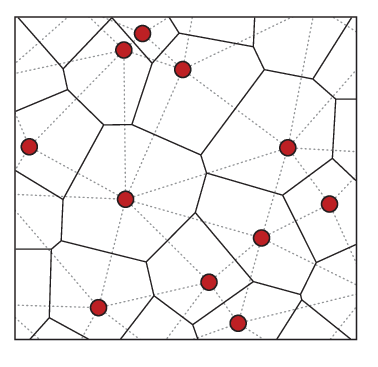
\includegraphics[width=0.4\textwidth]{Images/A-set-of-atoms-the-associated-Voronoi-tessellation-solid-lines-and-the-Delaunay.png}
    \caption[Voronoi tessellation.]{Example of Voronoi tessellation with highlighted nuclei.}
    \label{fig:voronoi}
\end{figure}


\subsection{Algorithm Steps}
\label{subsec:algsteps}
In this section, I will provide a detailed description of algorithm steps.
Suppose a latent field of labels $\Lambda_0:\mathcal{S}_0 \rightarrow \{1,\dots,L\}$ which is defined on the lattice $\mathcal{S}_0$. $\Lambda_0(\mathbf{x})$ is the true unknown label associated to the site $\mathbf{x}\in\mathcal{S}_0$, where $\mathcal{S}_0 \subset \mathcal{S}$ and $\mathcal{S}$ is a measurable subset of $\mathbb{R}^d$. In addition, suppose that a functional datum is observed in each site $\mathbf{x}\in\mathcal{S_0}$. In Algorithm \ref{alg:bvc} there is the pseudo code of the Bagging~-~Voronoi algorithm.

\begin{algorithm}
\scriptsize
    \caption{\footnotesize{Bagging Voronoi Classifiers}}
    \label{alg:bvc}
    \begin{algorithmic}
    \STATE \textbf{Bootstrap:}
    \STATE Initialize $B, n, p, K$. Choose a metric $d(\cdot,\cdot).$
    \FOR{$b:=1$ to $B$}
    \STATE{Randomly generate a set of nuclei $\Phi^b_n=\{\mathbf{Z}_1^b, \dots, \mathbf{Z}_n^b\}$ among the sites in $\mathcal{S}_0$}
    \FOR{$i=1$ to $n$}
    \STATE $\mathbf{Z}_i^b\sim\mathcal{U}(\mathcal{S}_0)$, where $\mathcal{U}$ is the uniform distribution on the lattice. Obtain a random Voronoi tessellation of $\mathcal{S}_0, \{V(\mathbf{Z}_i^b|\Phi_n^b\}^n_{i=1}$ by assigning each site $\mathbf{x}\in \mathcal{S}_0$ to the nearest nucleus $\mathbf{Z}_i^b$, according to the specified distance $d(\cdot,\cdot).$
    \ENDFOR
    \FOR {$i:=1$ to $n$}
    \STATE Compute the function $g_i^b$, acting as local representative, by summarizing information carried by the functional data associated to sites belonging to the $i$-th element of the tessellation $V(\mathbf{Z}_i^b|\Phi_n^b)$.
    \ENDFOR
    \STATE Perform dimensional reduction of the local representatives $\{g_1^b,\dots, g_n^b\}$ by projecting them on the space spanned by a proper $p$-dimensional scores vectors $\{\mathbf{g}_1^b,\dots, \mathbf{g}_n^b\}$, which are then clustered in $K$ groups according to suitable unsupervised method.
    \ENDFOR
    \STATE \textbf{Aggregation:} perform cluster matching
    \FOR {$k:=1$ to $K$}
    \FOR {$b:=1$ to $B$}
    \STATE indicate with $C_k^b$ the set of $\mathbf{x} \in \mathcal{S}_0$ whose label is equal to $k$, and match the cluster labels across bootstrap replicates, to ensure identifiability.
    \ENDFOR
    \ENDFOR
    \FOR {$\mathbf{x} \in \mathcal{S}_0$}
    \STATE Calculate the frequencies of assignment of the site to each of the $K$ clusters along iterations, \textit{i.e.}, $\pi_{\mathbf{x}}^k=\#\{b\in\{1,\dots,B\}:\mathbf{x}\in C_k^b\}/B, \forall k=1,\dots,K$
    \ENDFOR
    \end{algorithmic}
\end{algorithm} 


\paragraph{Step 1: Voronoi Tessellation} Select a set of points $\mathbf{x}\in\mathcal{S}$ as nuclei for the Voronoi tessellation. Thus, let $\Phi_n=\{\mathbf{Z}_1, \dots, \mathbf{Z}_n\}$ be a set of $n$ points in $\mathcal{S}$ sampled from a proper distribution $F$ defined on S: this will be the set of nuclei of the Voronoi tessellation. For each $\mathbf{Z}_i\in\Phi_n$ define the polyhedron
\begin{equation}
    \label{eq:polyedron}
    V\left(\mathbf{Z}_i \mid \Phi_n\right)=\{\mathbf{x}\in\mathcal{S} : d\left(\mathbf{x},\mathbf{Z}_i\right) \leq d\left(\mathbf{x}, \mathbf{Z}_j\right), \quad \text{for all}\quad \mathbf{Z}_j \in \Phi_n, i\neq j\}
\end{equation}
to be the closest Voronoi cell with nuclues $Z_j$ for the Voronoi tessellation induced by $\Phi_n$.
\paragraph{Step 2: Functional Local Representatives} Consider T, a bounded interval of $\mathbb{R}$ and a realization $f_{\mathbf{x}}:T\rightarrow \mathbb{R}$ of a functional random variable is observed in each site $\mathbf{x}$ of the lattice $S_0$. From the previous step, we got a Voronoi tessellation of the lattice $S_0$ which define random neighborhoods. For each element $V_i$ of the Voronoi tessellation, we sum up the information contained in the sub-sample $\{f_{\mathbf{x}}\}_{\mathbf{x} \in V_i}$ by estimating a functional local representative through a method that exploits spatial dependence of neighboring data. As example, the authors suggest to use weighted mean with a Gaussian kernel, but we can use any functional local representative we prefer, depending also on our needs and problem domain. For $i=1, \dots, n$ the functional local representative $g_i$ aforementioned is defined as
\begin{equation}
    \label{eq:gaussianmean}
    g_i(t)=\frac{\sum_{\mathbf{x}\in V_i}w^i_{\mathbf{x}}\cdot f_{\mathbf{x}}(t)}{\sum_{\mathbf{x}\in V_i}w^i_{\mathbf{x}}}
\end{equation}
where $w_{\mathbf{x}}^i$ is a Gaussian weight centered in $Z_i$ and decreasing with respect to $d\left(\mathbf{x}, \mathbf{Z}_i\right)$. Intuitively, we assume that spatial dependence between two sites decreases when the distance between them increases. The kernel covariance matrix is $\sigma^2\mathbb{I}_2$, where $\sigma=d_{max}/d_{min}$, being $d_{max}$ and $d_{min}$ the maximum and minimum distance between two nuclei of the tessellation, respectively. This choice connects $\sigma$ to the mean dimension of the tessellation element via an estimator of the elements mean diameter. The choice of $n$, which sets the tessellation dimension and thus the number of local representatives to be computed, has great influence on the algorithm behavior: in general, we have to find an optimal $n$ such that finds a good compromise between variance and bias. We will see two possible approaches for choose the optimal $n$ value in Section \ref{sec:bcv-cases}.

\paragraph{Step 3: Dimensional Reduction and Clustering} The third step of the algorithm aims at performing data dimensional reduction and at clustering the dimensionally reduced data. The most common tools used for dimensionality reduction of functional data is FPCA. For dimensional reduction of functional data, we need to find the best projection local representatives $\{g_1, \dots, g_n \}$ onto the space generated by a proper functional basis of finite dimension $p$. To choose the right dimension $p$, we can use the amount of variance explained by each functional principal component. "For instance, we could set a threshold, say 95\%, and keep the first $p$ principal components that account for a variance greater than or equal to 95\% of the total variance of the initial functional data. Alternatively, we could use the scree plot of the absolute amount of variance explained by each principal component and retain the $p$ components before the knee. This latter approach offers more freedom of choice to the analyst, thus a deep understanding of the problem domain becomes essential. We can repeat steps 1-3 $B$ times using a bootstrapping approach, where $B$ is arbitrary chosen. 

\paragraph{Step 4: Cluster Matching} The output of the $b$-th replicate of the bootstrap phase of the algorithm is a label assignment for each local representative estimated during the $b$-th run. All sites $\mathbf{x} \in V_i^b$ get the same label associated to the function local representative $g_i^b(t)$. To obtain a classification map of the lattice $\mathcal{S}_0$, we consider the frequency distribution of assignment of each site to each of the $K$ clusters along the $B$ replicates. To compute this frequency distribution we need in turn to assume that cluster labels $\{C_1^b, \dots, C_K^b\}$ are coherent along the $B$ replicates. More specifically, we want cluster labels $\{C_1^b, \dots, C_K^b\}$ to be coherent with $\{C_1^m\, \dots, C_K^m\}$, for all $m<b$ and $b\geq2$. This is obtained through cluster matching. Cluster matching is a set of techniques that allow us to keep different clustering algorithm outputs coherent. I will discuss a simple approach based on the use of contingency table. The algorithm looks for the label permutation that minimizes the total sum of the off-diagonal frequencies in the contingency table describing the joint distribution of sites along the classifications at two subsequent replicates. At the end of clustering matching, for each site $\mathbf{x}$ we will have a vector $\pi_{\mathbf{x}}^K=\left(P_1, \dots, P_K\right)$ where each $P_i, \quad i=1,\dots,k$ is the frequency the label $k$ was assigned to the site $\mathbf{x}$. The final label will be the label associated to maximum $P_k$. In other words, it is a majority voting process among the different replicates $b$.

\paragraph{Step 5: Evaluate Output} To have an overview of the statistical validity of the clustering just performed, we can use \textit{spatial entropy}. This concept is directly derived from the classical notion of entropy. Considering the frequency distribution vector $\boldsymbol{\pi}=(\pi_{\mathbf{x}}^1,\dots,\pi_{\mathbf{x}})^K$ of each site $\mathbf{x} \in \mathcal{S}_0$ to each of the $K$ clusters obtained after the bootstrapping step of the algorithm. The entropy associated site $\mathbf{x}$ classification in the site $\mathbf{x}\in\mathcal{S}_0$ is defined as
\begin{equation}
\mathbf{\eta}_{\mathbf{x}}=-\sum_{k=1}^K\pi_{\mathbf{x}^k}\cdot \log(\pi_{\mathbf{x}^k})
\end{equation}
which assumes the minimum value 0 when there is an $r$ such that $\pi_{\mathbf{x}}^r=1$ while $\pi_{\mathbf{x}}^k=0$ for all $k\neq r$ and maximum value $\log(K)$ when $\pi_{\mathbf{x}}^k=\frac{1}{K}$ for $k\in\{1,\dots,K\}$. We can see spatial entropy as a measure of the disorder of the frequency of assignment the site $\mathbf{x}\in\mathcal{S}_0$ to cluster $k$. Moreover, we can compute the \textit{average normalized entropy} to have a global evaluation index of the clustering performed. Average normalized entropy is defined as
\begin{equation}
\label{eq:avgentropy}
    \eta^K=\frac{\sum_{\textbf{x}\in\mathcal{S}_0}\eta_{\mathbf{x}}^K}{\log(K)\cdot |\mathcal{S}_0|}
\end{equation}
From \ref{eq:avgentropy} we can appreciate how the index has been normalized to maximum value $\log(K)$ in order to allow comparison over different choices of $K$. An other possible index for evaluating a classification in the ratio
\begin{equation}
    \label{eq:theta}
    \theta=\frac{tr(B)}{tr(B)+tr(W)}
\end{equation}
where $B$ and $W$ are the final between and within cluster sum of squares matrix, respectively. This index can be seen as the percentage of variance explained by splitting the observations in clusters.



% <<< End of Bagging Voronoi Clustering Algorithm

% Succesful case of the algorithm >>>
\section{Successful Case Studies in Clustering Algorithm Application}
\label{sec:bcv-cases}
In this section, we will discuss two examples of how the algorithm outlined in the previous section has been successfully applied in two completely different domains: the clustering of irradiance data performed in \citeauthor{secchi_bagging_2013} \citeyear{secchi_bagging_2013} and the analysis of spatio-temporal mobile phone data performed in \citeauthor{secchi_analysis_2015} \citeyear{secchi_analysis_2015}. In the first case, the goal is to cluster irradiance data, while in the second case is to find some surfaces in order to explain human activity in space and time. The purpose of this section is to address any potential questions or uncertainties the reader may still have regarding the use of Algorithm \ref{alg:bvc} and show some possible ways to approached this analysis.
\subsection{Clustering of Irradiance Data}
\label{subsec:irradiance}
Insolation refers to the amount of solar radiation energy captured on a specific surface area over a set time period. Typically, it is computed as average irradiance in kilowatt-hours per square meter per day (\unit{\kilo\watt.h/\metre^2.day}). Authors focused on direct insolation, which pertains to the solar irradiance measured at a particular location on Earth with a surface facing directly towards the sun's rays, omitting diffuse insolation. Diffuse insolation refers to the solar energy scattered or reflected by atmospheric components overhead. The value of direct insolation is derived from the solar constant minus the atmospheric reductions from absorption and scattering. While the solar constant is influenced by factors like Earth's distance from the sun and solar cycles, the losses are contingent on factors such as the time of day (which affects the light's path through the atmosphere based on the sun's elevation angle), cloud coverage, atmospheric moisture, and other contaminants. Author's goal was to identify areas of the planet which are optimal with respect to the positioning of solar power collectors by considering parameters, which depend on direct insolation. The data available for the analysis consists of vectors in $\mathbb{R}^{12}$ indexed by each site of the lattice. Sites are located on a non-uniform lattice $\mathcal{S}_0=\bigcup_{\lambda \in Z_{\mathbf{1}};\theta \in Z_{\mathbf{2}}}A_{\lambda\theta}$ where $Z_{\mathbf{1}} = \{ -180, -179, \dots, 178, 179\}$ and $Z_{\mathbf{2}} = \{ -66, -65, \dots, 65\}$: each element $A_{\lambda\theta}$ is the portion of the earth surface which is included between the meridians at longitude $\lambda$ and $\lambda + 1$ in degrees, and between the parallels at latitude $\theta$ and $\theta + 1$ in degrees. This lattice is of course non-uniform, and includes 47,520 worldwide non-polar districts. In each site, the 12 measures correspond to the values of the monthly maximum energy deficit with respect to the monthly average. Both the maximum and the average values are computed over the 22 years time period from July 1983 to June 2005. For each site, authors obtained a functional datum $Y_{\lambda,\theta}(t)$ by smoothing $\{Y_{\lambda\theta}^1, \dots, Y_{\lambda\theta}^12\}$ with a Gaussian kernel with bandwidth equal to 1.5, where $Y_{\lambda\theta}^\nu$ is the irradiance data for each month. The authors chose to use a Gaussian isotropic kernel to compute the weighted average local representatives. They selected the first $p=3$ functional principal components since that with only these 3 components the proportion of explained variance was greater than 95\%. For classifying the scores of the $n$ representatives, they employed the K-Means algorithm with the $L^2$ semi-metric induced by the principal components.
\begin{figure}
    \centering
    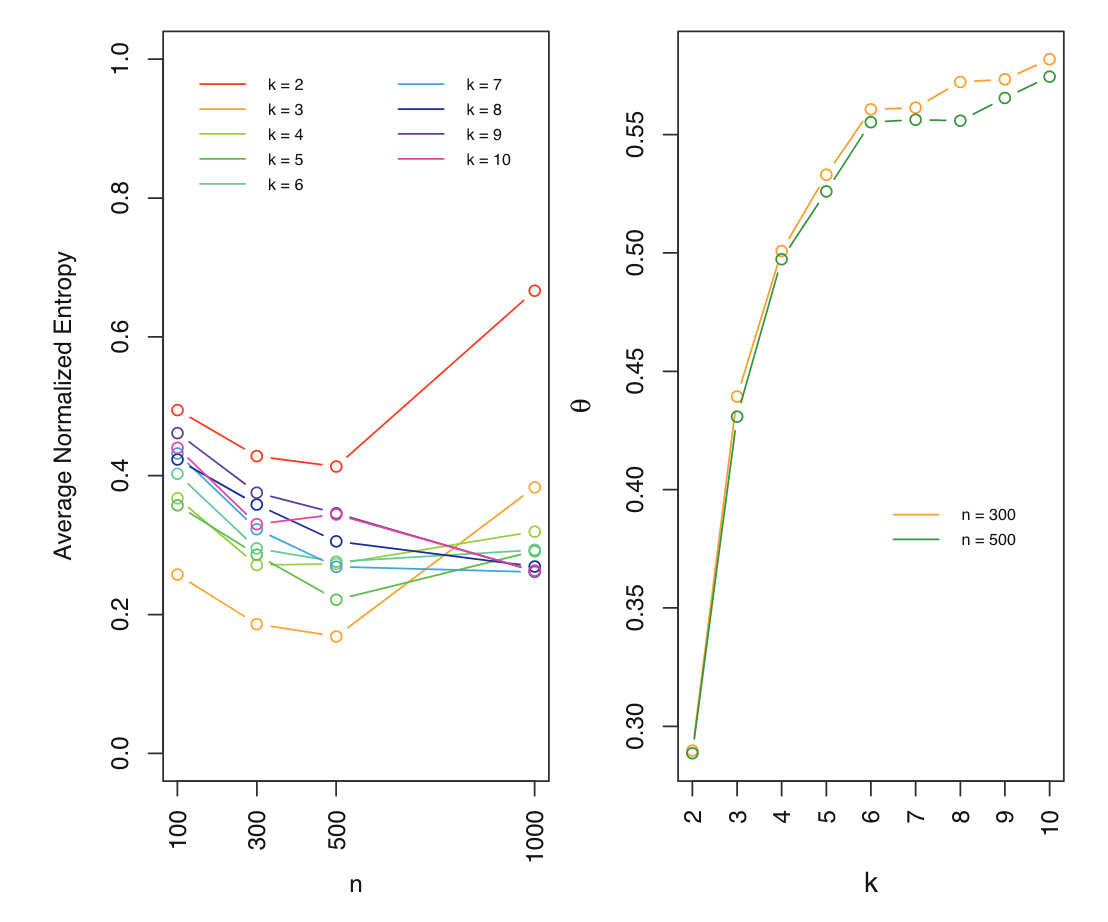
\includegraphics[scale=0.5]{Images/baggingscreeplot.png}
    \caption[Result on irradiance data.]{Algorithm performances with irradiance data. On the left, average normalized entropy, on the right the index $\theta$ \cite{secchi_bagging_2013}.}
    \label{fig:baggingscreeplot}
\end{figure}
Subsequently, as with all classical clustering problems, they performed the clustering multiple times in order to obtain the scree plot shown in Fig. \ref{fig:baggingscreeplot} and to select the optimal number of clusters, $K$. Additionally, with this specific algorithm, it was also necessary to determine the optimal number of nuclei, $n$, for the initial Voronoi tessellation. To find the scree-plots shown in the above figure, the number of bootstrap replications was set at $B=100$, and the parameters $n$ and $K$ were varied. The optimal choice for these two parameters was made by using average normalized spatial entropy, the index $\theta$, and the normalized spatial entropy map in conjunction. Starting from the scree-plot of average normalized entropy in Fig. \ref{fig:baggingscreeplot}, we can see that for $n=500$, we have two local minima, specifically for $K=3$ and $K=5$. From the same figure, we can observe that the graph of $\theta$ suggests that the number of clusters $K=6$ appears to be the most reasonable. Indeed, using $K=7$ would not be a good choice, as it would not enhance the classification obtained. Consequently, the classification should yield good results for $K=5$ and $K=6$. This was also confirmed by the maps of the normalized entropy, shown in Fig. \ref{fig:irrentropy}.
\begin{figure}[H]
    \centering
    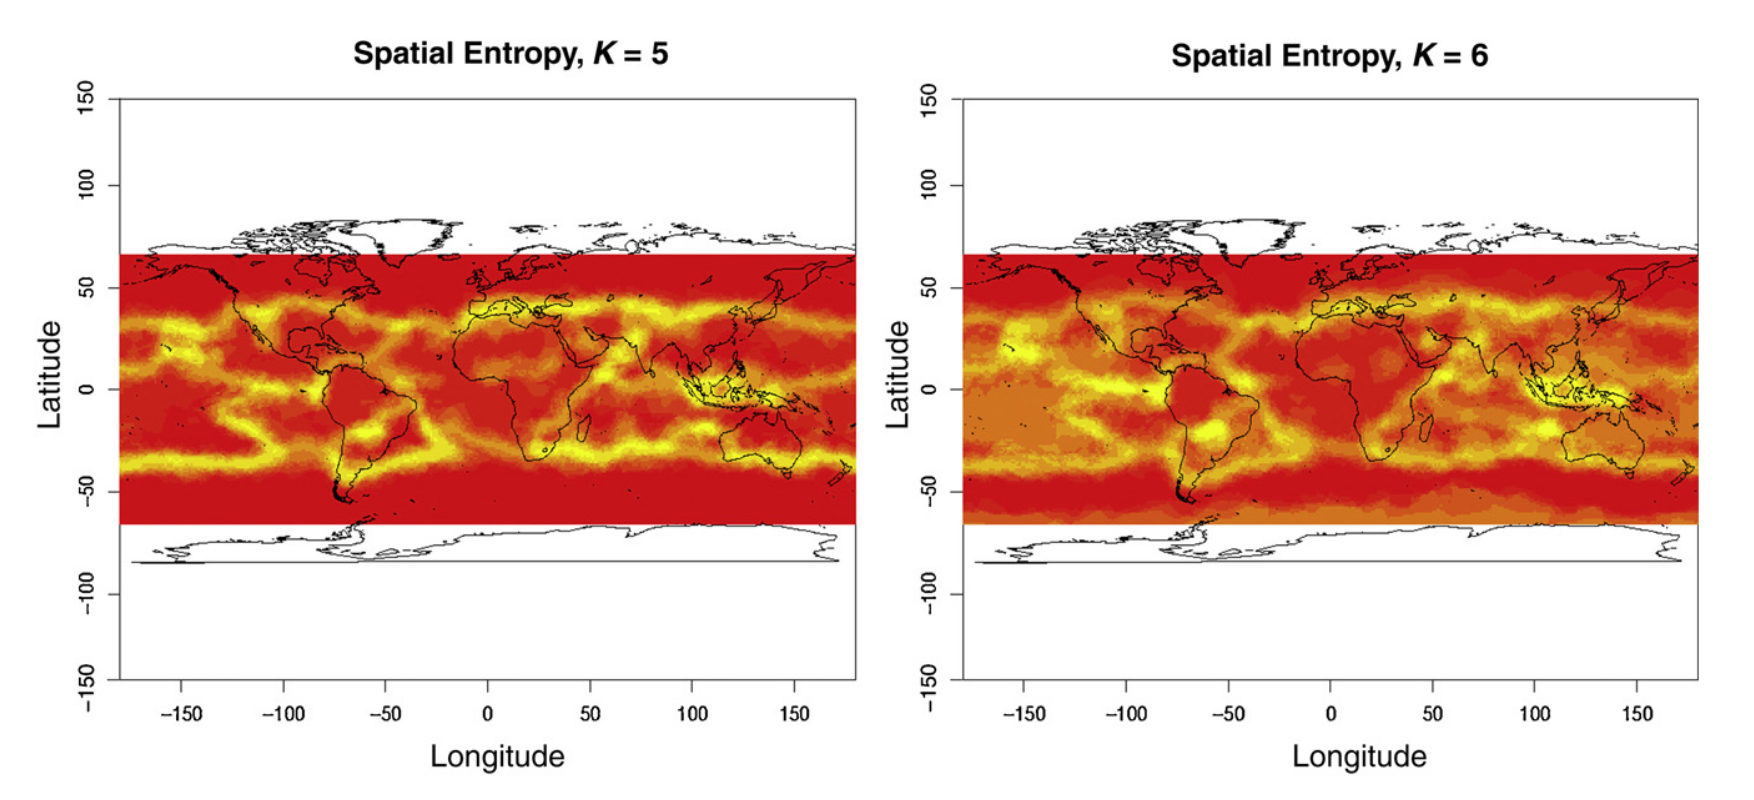
\includegraphics[scale=0.5]{Images/irrentropy.png}
    \caption[Spatial entropy for irradiance data.]{Normalized spatial entropy maps associated to the classification with K = 5 (left) and K = 6 (right). Colors from red to white correspond to values from 0 to 1; higher values identify areas where classification is more uncertain. \cite{secchi_bagging_2013}.}
    \label{fig:irrentropy}
\end{figure}
The final choice $K=5$ was made looking at maps in Fig. \ref{fig:irrentropy}, which tell us that for $K=5$ the classification is more robust, and from the fact that with $K=5$, the algorithm identified different homogeneous macro-areas which seem interpretable in terms of observed phenomenon.  In Fig. \ref{fig:resbagging} there are the final cassifications for irradiance data. The two classifications are not in contrast, but somehow support each other. Now, as mentioned earlier, we can take advantage of the functional nature of the data to derive additional insights that wouldn't be possible with traditional clustering algorithms. For instance, the fact that the red cluster exhibits a non-seasonal pattern that remains consistent throughout the year, or how the green and yellow clusters have opposite seasonal patterns. The advantage of using $K=6$ is the fact that with orange cluster, we can identify some sites characterized by a very high seasonality. To conclude, it's noteworthy to observe that spatial entropy is systematically higher near the boundary between two different clusters. This is due to the fact that the functional data is actually spatially dependent, and hence data near the boundaries are more challenging to cluster.
\begin{figure}
    \centering
    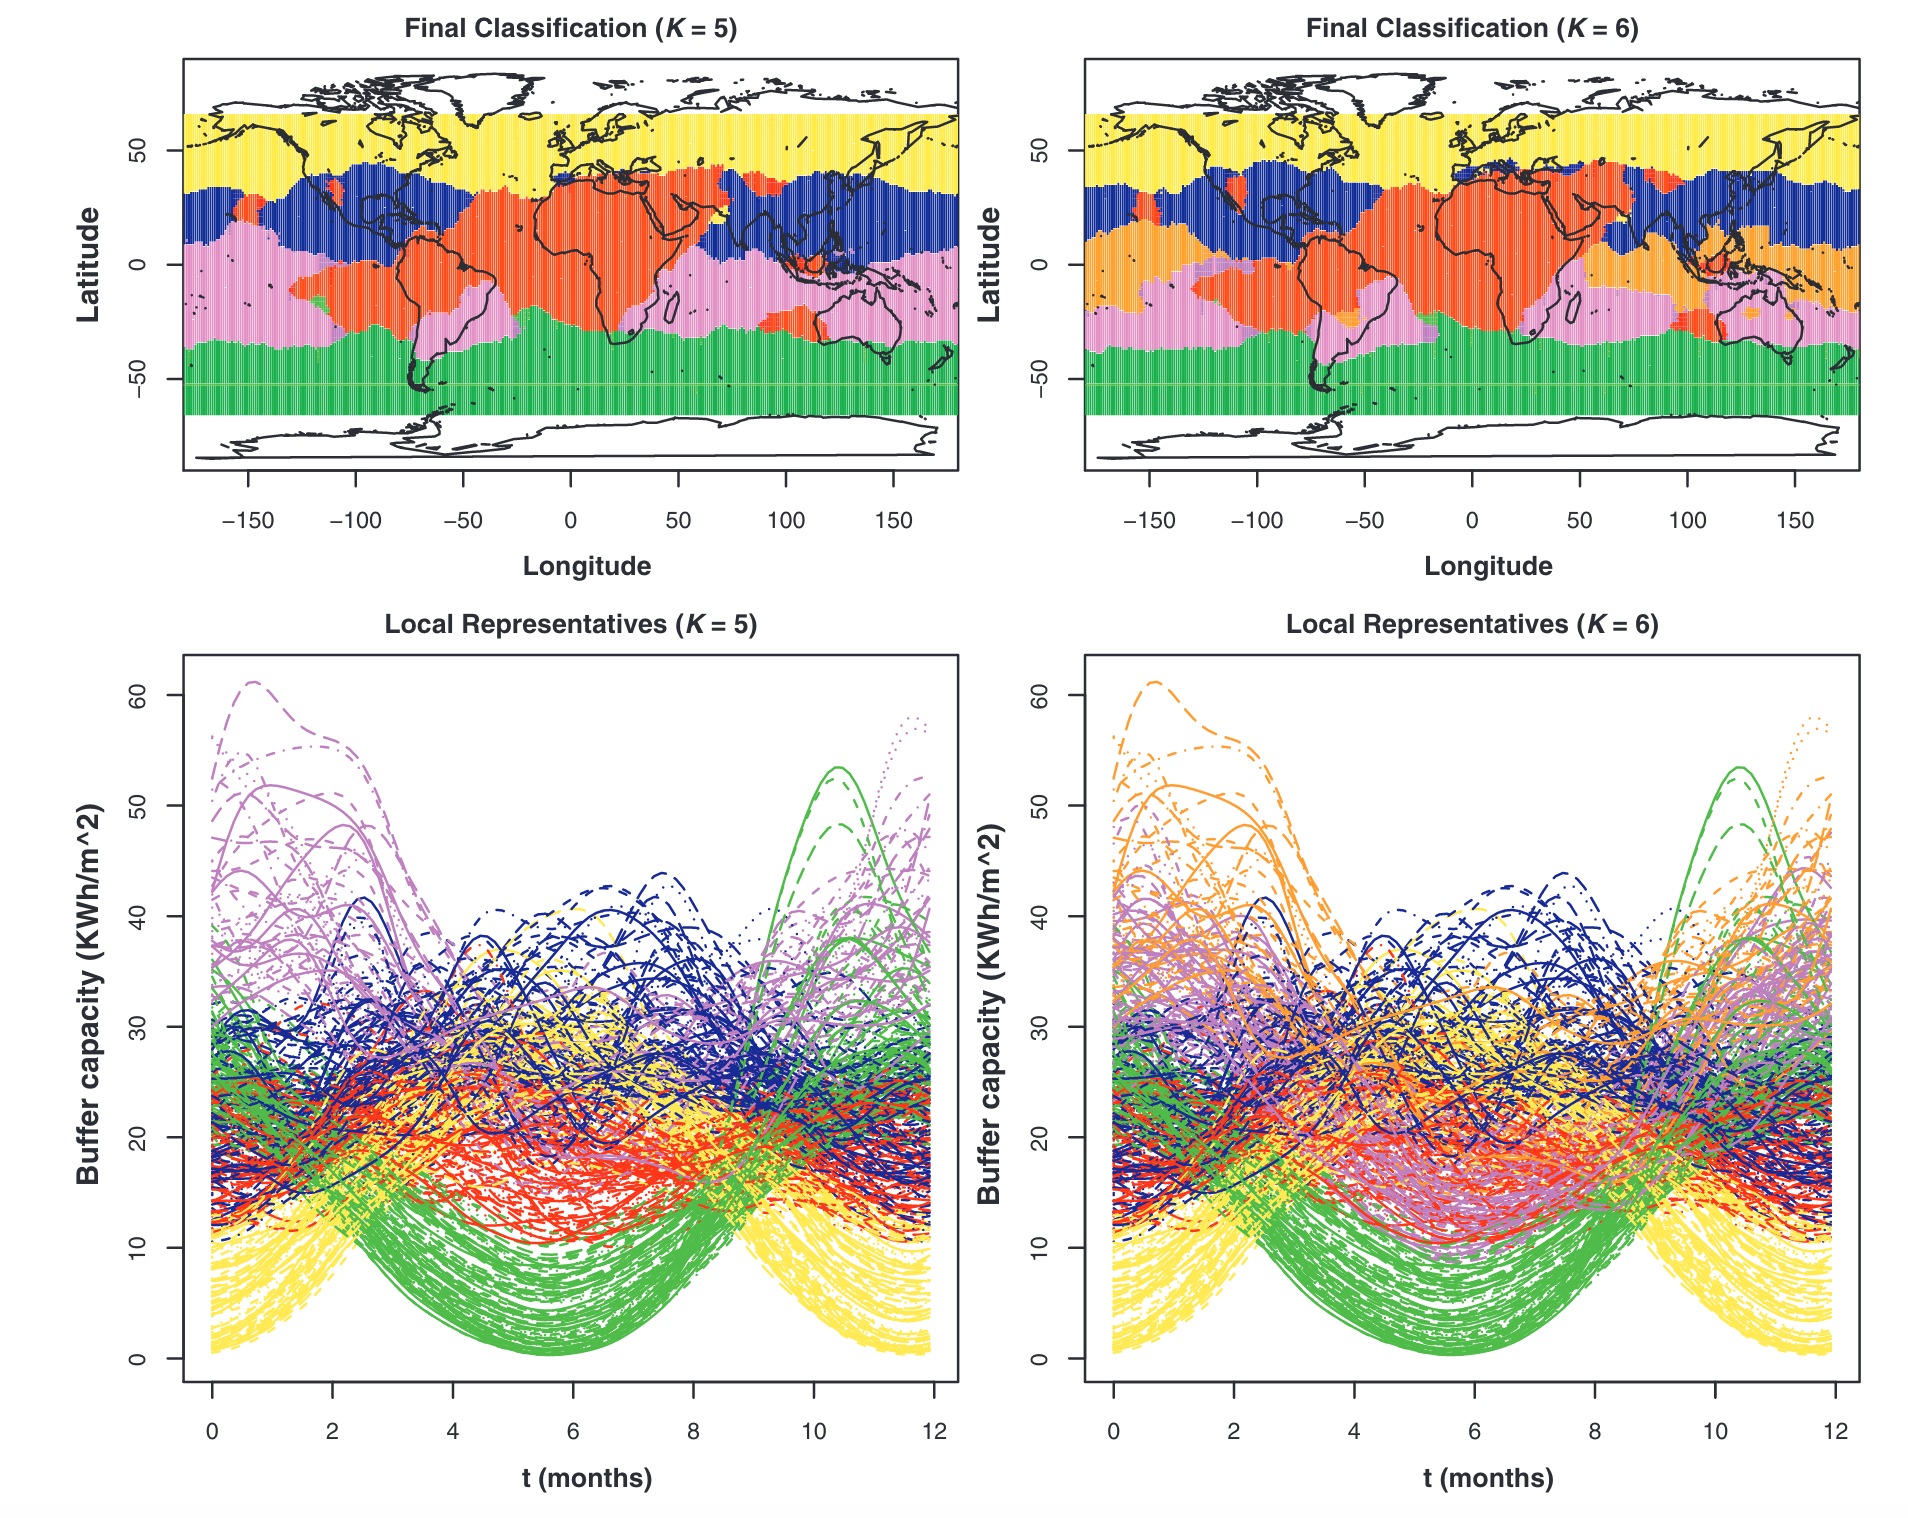
\includegraphics[scale=0.4]{Images/resbagging.png}
    \caption[Classification of irradiance data.]{In the top panels, final classification maps obtained via a majority vote on frequencies of assignment, and by setting $K = 5$ (left) or $K = 6$ (right).In the bottom panels, a set of functional local representatives obtained with $n = 500$ in one of the iterations of the algorithm and clustered with $K = 5$ (left) and with $K=6$ (right). From \citeauthor{secchi_bagging_2013} \citeyear{secchi_bagging_2013}.}
    \label{fig:resbagging}
\end{figure}
I think that the parallelism between irradiance ~data~-~planet and temperature ~profiles~-~print ~plate seems straightforward and fairly clear. So, it's reasonable to believe that an application in additive manufacturing could lead to significant advancements..
\subsection{Analysis of Spatio-Temporal Mobile Phone Data in Milan}
\label{subsec:mobilephonemilan}
I have chosen to present this example to illustrate to the reader the flexibility of the previously discussed algorithm. It demonstrates how the method can adapt with different data dimensionality reduction techniques and how a Fourier basis can be employed to represent functional data exhibiting certain seasonality, as is the case with lattice structures in Section. \ref{subsec:devcell}.
In \citeauthor{secchi_analysis_2015} \citeyear{secchi_analysis_2015}, authors examined high-dimensional, geo-referenced mobile-phone usage data from Milan's urban area to discern patterns of activity within the city over time. The goal was to identify specific urban zones with similar temporal patterns, which could indicate specific activities or events in those areas. To achieve the goal, they decided to use the algorithm explained in Section \ref{sec:bvc} coupled with treelet analysis (I'll explain what it is in just a moment). 
The data available for analysis are from Telecom Italia. In this dataset, the metropolitan city of Milan is divided into a uniform lattice $\mathcal{S}_0$ consisting of 97x109 sites. In each site, the average number of mobile phones simultaneously using the network for calling is provided every 15 minutes over a span of 14 days. This quantity is called Erlang and it is defined as
\begin{equation}
    \label{eq:erlang}
    E_{\mathbf{x}j}=\frac{1}{15}\sum_{q=1}^Q \left| T_{\mathbf{x}j}^q \right|
\end{equation}
where $T_{\mathbf{x}j}^q$ indicates the time interval in which the $q$-th mobile phone is using the network for calling while moving within site $\mathbf{x}$ and during the $j$-th quarter of an hour. The Erlang data was recorded every quarter of an hour, from March 18th, 2009, 00:15, till March 31st, 2009, 23:45. Fig. \ref{fig:secchino} there is an example of an Erlang profile.
\begin{figure}[H]
    \centering
    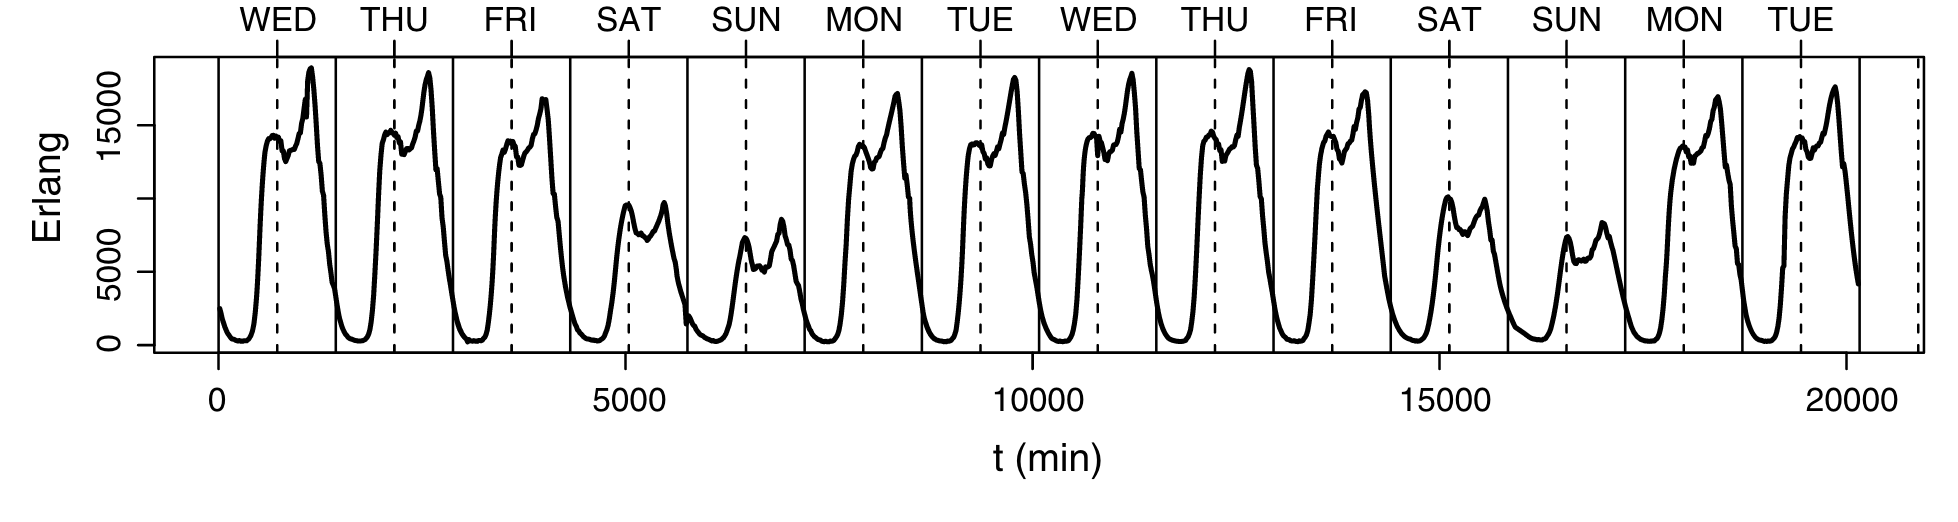
\includegraphics[scale=0.43]{Images/secchierlang.png}
    \caption[Erlang profile.]{Erlang profile for a site in the lattice $\mathcal{S}_0$ \cite{secchi_analysis_2015}.}
    \label{fig:secchino}
\end{figure}
However, for some sites of the lattice, Erlang profiles had some missing values, and in some instances, they were entirely missing. Therefore, after the data cleaning phase, the authors decided to focus only on a non-uniform time grid of $p = 1,308$ elements, each element of the time grid being relative to a quarter of an hour for which an Erlang measurement has been observed in at least one site of the lattice. In Algorithm \ref{alg:bvc} for dimensional reduction of functional data, FPCA was suggested. While FPCA stands as an effective technique for identifying optimal subspaces to represent data, it has a limitation in its global approach, making it less appropriate for multi-resolution analysis. This is primarily because its basis elements typically involve a linear combination of all foundational variables. So, authors decided to use a treelet basis, introduced in \citeauthor{lee_treelets--adaptive_2008} (2008). For this specific case, since the data exhibits an evident seasonality, authors decided to use a Fourier basis with a period equal to 1 week. Thus, the reconstructed functional form of the Erlang profile for site $\textbf{x} \in \mathcal{S}_0$ is a function $E_{\textbf{x}(t)}$ such that:
\begin{equation}
    E_{\textbf{x}}(t)=\frac{c_0^{\textbf{x}}}{2} + \sum_{h=1}^H \left[a_h^{\textbf{x}}\cos \left( h\omega t\right) + b_h^{\textbf{x}}\cos \left( h\omega t\right) \right]
\end{equation}
where $t \in \left[ 0; T\right]$, $\omega = 2\pi/T$ and $T=60 \times 24 \times 7$ is the period expressed in minutes. To choose the optimal basis dimension $H$, we can use the power spectrum associated to the site~-~wise smoothing of the Erlang data with a Fourier basis of large dimension $H = 200$. The power spectrum of the Fourier expansion of a signal represents the amplitude of the signal as a function of the frequency, and at the $h$-th frequency it is related to the amplitude of the $h$-th harmonic

\begin{equation}
    \label{eq:spectrum}
    P_{\mathbf{x}}(h)=\sqrt{(a^{\mathbf{x}}_h)^2 + (a^{\mathbf{x}}_h)^2}
\end{equation}

Thus, the more the $h$-th harmonic is relevant in the explanation of features occurring in the data, the more $P_{\mathbf{x}}(h)$ will be large. From the spectrum in Fig. \ref{fig:fantasmino}, we can see that local maximum happening at multiple of 7 (the dotted lines), while for $H >100\omega$, power spectre becomes almost negligible.

\begin{figure}[H]
    \centering
    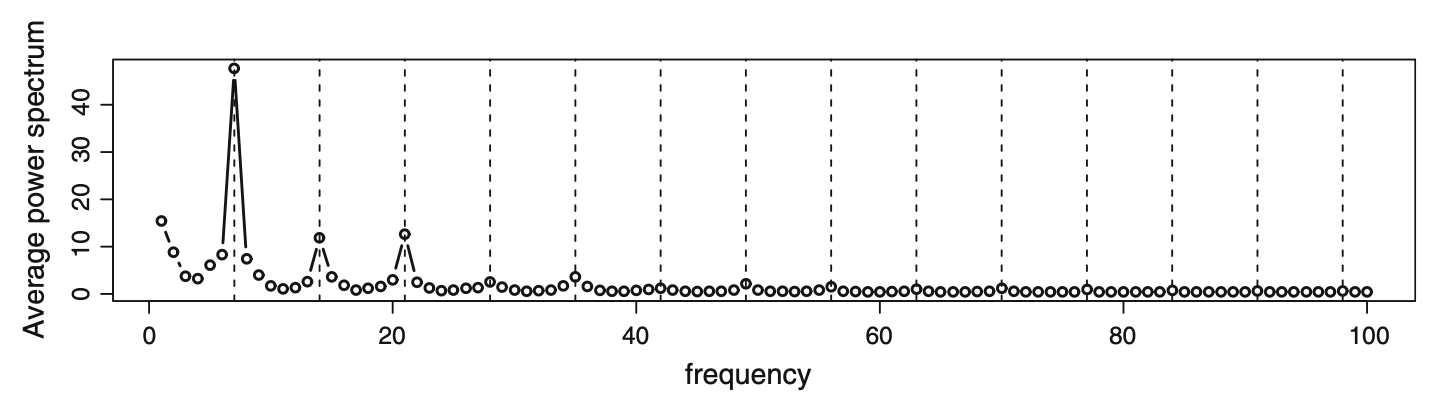
\includegraphics[scale=0.6]{Images/fantasmino.png}
    \caption[Spectrum of Erlang data.]{Average power spectrum $P(h)$ obtained via site-wise smoothing of the Erlang measures with a Fourier basis of dimension $H = 200$. Only the values of $P(h)$ for$ h = 1, \dots, 100$ are shown in the plot. Dotted vertical lines are drawn for multiples of 7 \cite{secchi_analysis_2015}.}
    \label{fig:fantasmino}
\end{figure}

As did in Section \ref{subsec:irradiance}, the metric $d(\cdot, \cdot)$ used is Euclidean distance, the total number of bootstrap $B=50$, and the dimension $n$ of the Voronoi tessellation ranging from 50 to 1250. As we already know, the optimal $n$ will be found by using the scree plot.


\subsection{Deviation Index in Lattice Structure Cells}
\label{subsec:devcell}
In previous section, I have chosen to provide an example of how functional data and clustering algorithms can be used to conduct a layer-wise temperature profile analysis. However, these concepts can be readily adapted to other scenarios, including, for instance, particular application in three dimensions. In this section, I want to go beyond the primary domain of the thesis. I want to suggest how the algorithm could also be leveraged for the classification of functional data in three dimensions. A possible application in three dimensions could be the clustering of functional data regarding the deviation of cell profiles in lattice structures. Recall that in 3 dimension, Voronoi regions are represented as polyhedra, like in Fig. \ref{fig:3dvoronoi}.

\begin{figure}[H]
    \centering
    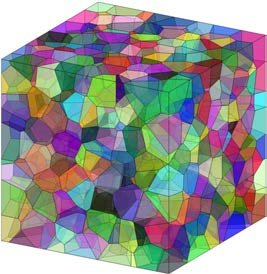
\includegraphics[scale=0.43]{Images/3D-Voronoi-tessellation-with-1000-grains-unit-cell-with-its-internal-grains-not.png}
    \caption[3d Voronoi tessellation.]{An example of a Voronoi tesselation in 3d.}
    \label{fig:3dvoronoi}
\end{figure}

In \citeauthor{colosimo_complex_2022} (2022), the authors aim to compare the nominal slices with the actual slices measured through x-ray computed tomography of a lattice structure composed of 64 dodecahedron unit cells of size \SI{10}{\milli\metre} within a specimen of $40 \times 40 \times 40$ \unit{\milli\metre}. Subsequntely, the 2D image of the as-built single cell and as-designed one were compared, slice by slice, in order to compute the deviation index. Given a pair of images that correspond to the $z-$th slice of the as-designed cell and the $z-$th slice of the as-built cell, let $i_{u,v,z}(\text{as.designed}$ and let $i_{u,v,z}(\text{as.build}$ be the intensities of $(u,v)^{th}$ pixel in the as-designed slice and in the as-built slice, respectively. In Fig. \ref{fig:slices} there are some examples of the procedure. A superimposition of these two images leads to four possible cases:
\begin{itemize}
    \item Region 1: pixels in which both $i_{u,v,z}(\text{as.designed})=0$ and $i_{u,v,z}(\text{as.build})=0$, i.e., pixels where material is present in both the images.
    \item Region 2: pixels in which both $i_{u,v,z}(\text{as.designed})=1$ and $i_{u,v,z}(\text{as.build})=1$, i.e., pixels that correspond to the background in both the images.
    \item Region 3: pixels in which both $i_{u,v,z}(\text{as.designed})=0$ and $i_{u,v,z}(\text{as.build})=1$, i.e., pixels where material is present in the as-designed slice but not in the as-built slice (i.e., less material has been produced than indicated in the CAD model)
    \item Region 4: pixels in which both $i_{u,v,z}(\text{as.designed})=1$ and $i_{u,v,z}(\text{as.build})=0$, i.e. pixels where material is present in the as-built slice but not in the as-designed slice (i.e., more material has been produced than indicated in to the CAD model).
\end{itemize}


\begin{figure}
    \centering
    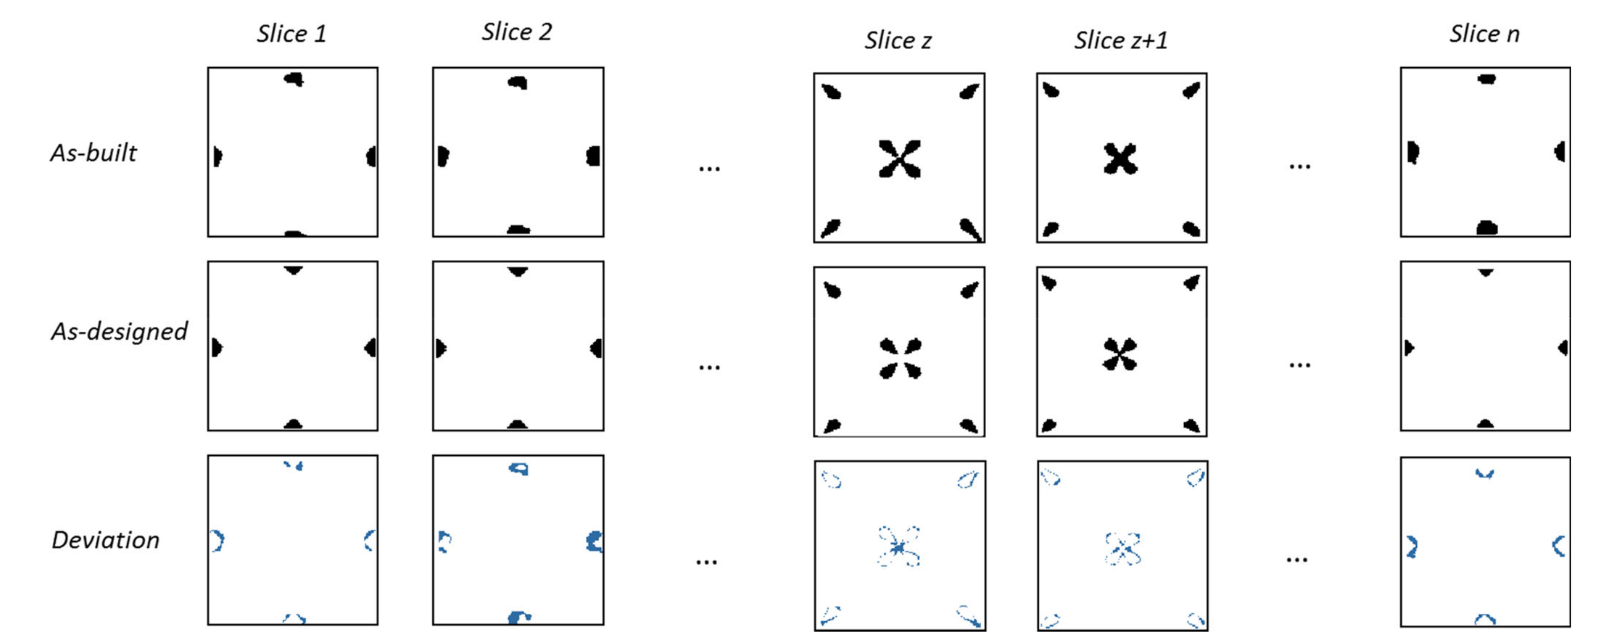
\includegraphics[scale=0.5]{Images/slicescolosimo.png}
    \caption[Deviation index.]{Example of as-built (top row) and as-designed (central row) slice images at different z heights with the corresponding deviation (bottom row) \cite{colosimo_complex_2022}. }
    \label{fig:slices}
\end{figure}


The overall number of pixels that belong to the union of region 3 or region 4 is the number of pixels for which $i_{u,v,z}(\text{as.build}) - i_{u,v,z}(\text{as.designed}) \neq 0$. So the \emph{deviation index} for the cell $(i,j,k)$ is defined as
\begin{equation}
\label{eq:deviationindex}
\delta_{i, j, k}(z)= \sum_{u=1}^p \sum_{v=1}^p \mathcal{I}\left(i_{u, v, z}(\text { as.built })\right. -i_{u, v, z}(\text { as.designed })\neq 0)_{i, j, k},
\end{equation}
where $\mathcal{I}$ is the indicator function, that is 1 if the condition in brackets is true and 0 otherwise.
After calculating the deviation index for each cell, the authors suggest using a cubic B-splines basis to fit a functional profile on the deviation index as a function of the slice position along cell z-axis. The position of the knots was chosen to eliminate the first and second discontinuity present in the deviation profiles, resulting from the typical trabecular structure of lattice designs. Fixed knots were then placed at the discontinuities of the as-designed geometry. Subsequently, intermediate knots were added iteratively, until a knee in the mean squared error (MSE) scree plot of the B-spline model residuals was identified.
At the conclusion of step 5 in Fig. \ref{fig:colosimofunctional}, as outlined in the article, we will have 64 functional profiles, one for each cell. These profiles and the centroid of each cell in a lattice in $\mathbb{R}^3$ and will be the input for the classification algorithm described in Section \ref{sec:bvc}. In doing so, we could identify if there are critical areas within the lattice where cells exhibit similar anomalous behavior. Coupled with the ability to quantify the magnitude of the defect using the functional profiles, this could lead to a deeper understanding of the lattice structure's behavior and determine whether, despite its imperfections, it remains fit for its intended use. Indeed, localized geometric and dimensional deviations of the unit cells might adversely affect the structure's elastic modulus and compressive strength \cite{colosimo_complex_2022}.

\begin{figure}
    \centering
    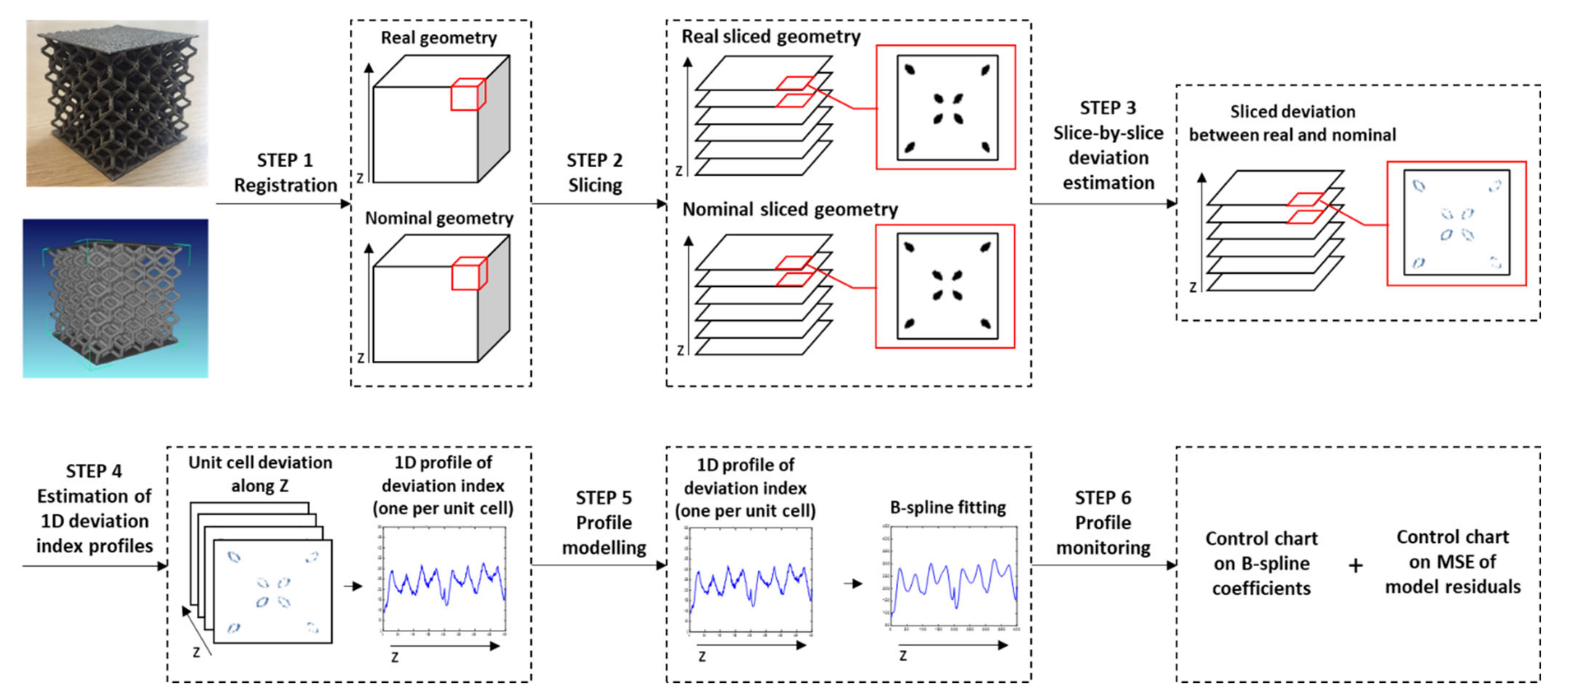
\includegraphics[scale=0.5]{Images/colosimosplines.png}
    \caption[Functional control chart in complex geometries.]{Schema of the proposed methodology in \cite{colosimo_complex_2022}. The output of step 5 would be the input for the classification algorithm.}
    \label{fig:colosimofunctional}
\end{figure}
% <<< End of Succesful case of the algorithm


%>>> Simulation Study
\section{Simulation Study}
\label{sec:simstudy}
\textcolor{red}{Se riesco a fare una simulazione con esito positivo la inserisco.} I dati che mi servono per fare la simulazione posso prenderli da qua \cite{anandan_kumar_faster_2021, burkhardt_thermo-mechanical_2022}.
% <<< End of Simulation Study

%As we will see in Section \ref{sec:bvc}, the number $K$ of clusters is an input of the algorithm, making hierarchical clustering not suitable for our purposes. But before delving into the algorithm's description, I also want to explain the concept of \textit{bagging} for clustering. It is based on the concept of bootstrapping. Bootstrapping is a resampling technique that helps in finding more reliable results from a clustering algorithm. In the algorithm, we will perform multiple clustering "rounds" in order to find a frequency distribution of the belongings of the observation to a specific cluster. The final cluster label for each observation will be the "most probable correct result" by majority voting.